\documentclass[a4paper,12pt]{report}
\addtolength{\oddsidemargin}{-1.cm}
\addtolength{\textwidth}{2cm}
\addtolength{\topmargin}{-2cm}
\addtolength{\textheight}{3.5cm}
\newcommand{\HRule}{\rule{\linewidth}{0.5mm}}
\setcounter{secnumdepth}{6}
\setcounter{tocdepth}{4}
\makeindex

\usepackage{longtable}
\usepackage{graphicx}
\usepackage{makeidx}
\usepackage{hyperref}
\usepackage{verbatim}
\usepackage{placeins}
\usepackage{float}
\usepackage{titlesec}

\makeatletter
\newcounter{subsubparagraph}[subparagraph]
\renewcommand\thesubsubparagraph{%
  \thesubparagraph.\@arabic\c@subsubparagraph}
\newcommand\subsubparagraph{%
  \@startsection{subsubparagraph}    % counter
    {6}                              % level
    {\parindent}                     % indent
    {3.25ex \@plus 1ex \@minus .2ex} % beforeskip
    {-1em}                           % afterskip
    {\normalfont\normalsize\bfseries}}
\newcommand\l@subsubparagraph{\@dottedtocline{6}{10em}{5em}}
\newcommand{\subsubparagraphmark}[1]{}
\makeatother

\hypersetup{
    colorlinks=true,
    linkcolor=blue,
    filecolor=magenta,      
    urlcolor=cyan,
}


% define the title
\author{Ambitious Design}
\title{ Software User Manual}
\begin{document}
\setlength{\parskip}{6pt}

% generates the title
\begin{titlepage}

\begin{center}
% Upper part of the page           


\includegraphics{willburg.png}\\
\textsc{\LARGE Willburg Outdoor PTY(ltd.)}\\[1.5cm]


\includegraphics[height=8cm]{ad.jpg}\\
\textsc{\Large Smart Image Identifier }\\[1.0cm]
\textsc{\Large Version 1.0 }\\[0.5cm]
% Title
\HRule \\[0.4cm]
{ \huge \bfseries  Software User Manual}\\[0.4cm]
\HRule \\[0.4cm]
% Author and supervisor
\begin{minipage}{0.4\textwidth}
\begin{flushleft} \large
\emph{Project Team:}\\
Stephen {Swanepoel}
\end{flushleft}
\end{minipage}
\begin{minipage}{0.4\textwidth}
\begin{flushright} \large
\emph{} \\
u11032091
\end{flushright}
\end{minipage}
\begin{minipage}{0.4\textwidth}
\begin{flushleft} \large
Dian {Veldsman}
\end{flushleft}
\end{minipage}
\begin{minipage}{0.4\textwidth}
\begin{flushright} \large
\emph{} \\
u12081095
\end{flushright}
\end{minipage}

\end{center}
\end{titlepage}
\footnotesize
\normalsize

\renewcommand{\thesection}{\arabic{section}}
\newpage
\tableofcontents
\newpage

\begin{center}
\textsc{\LARGE User Manual}\\[1.5cm]
\end{center}

\section{General Information}
\subsection{System Overview}
Smart Image Identifier is human recognition software written for Willburg to provide real-time processing of images on their server to assist in the improvement of security. The system is completely autonomous and thus has no user interaction, it is just system-to-system communications. 
\newline\newline
When an image is pushed to the server, Smart Image Identifier retrieves the image, processes it and sends an appropriate response back to the server

\subsection{System Configuration}

\subsection{Installation}
	\subsubsection{Install Eclipse}
	The easiest way to build the dispatcher from source is using Eclipse Neon. Eclipse Neon is a
	development environment and is open-source software. The latest version of this software can
	be obtained at https://www.eclipse.org/downloads/. After the download is completed, install
	the software using the instructions provided by the installer.
	
	\subsubsection{Importing the project}
	In Eclipse, click File, Import, General, finally, select, Existing Projects into Workspace and click
	Next. \newline\newline
	Select root directory, click Browse, locate the given project folder, finally, select Finish.
	
	\subsubsection{Setting system environment variables}
	Setting of environment variables is necessary for your system to detect the OpenCV framework
	which was used for developing Smart Image Identifier.
	
	\newpage
	Lets get started
	
	\begin{itemize}
		\item Step:1	\linebreak
		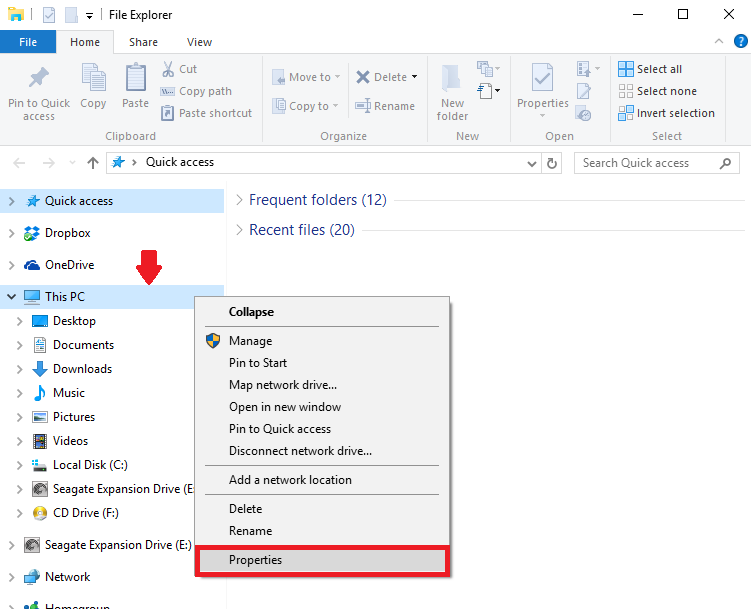
\includegraphics[height=8cm]{001.png}\\
		\linebreak
		Open File Explorer, right click on This PC (Yours may be named otherwise), click Properties
		\item Step:2	\linebreak
		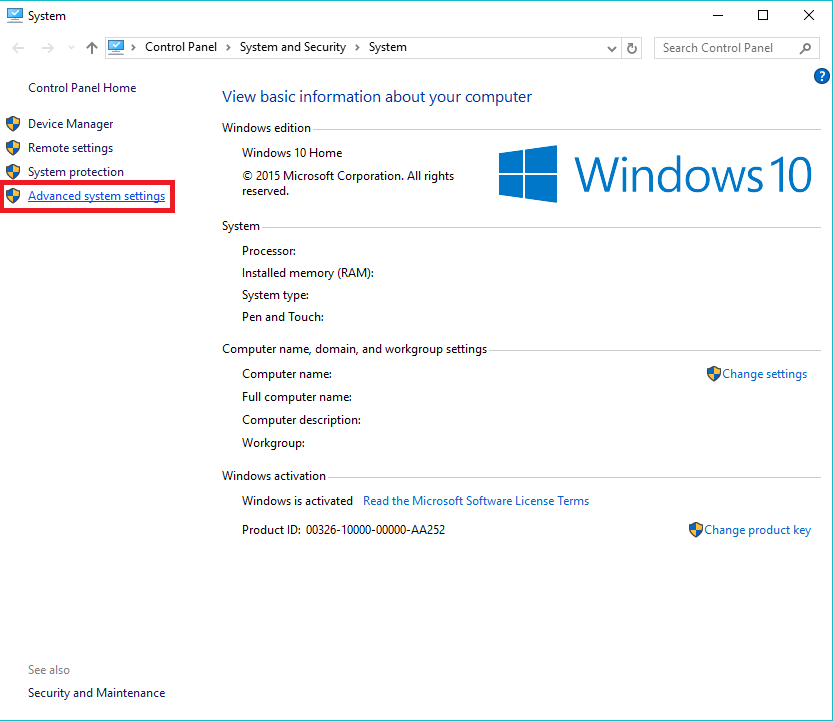
\includegraphics[height=8cm]{002.png}\\ 
		\linebreak 
		On the left hand panel select Advanced System Settings.
		\pagebreak
		\item Step:3	\linebreak
		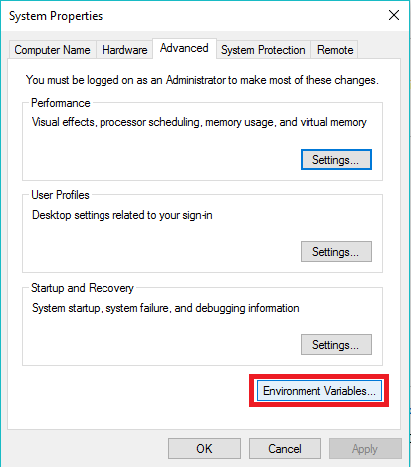
\includegraphics[height=8cm]{003.png}\\
		\linebreak
		Click Environment Variables located at the bottom of the window.
		\item Step:4	\linebreak
		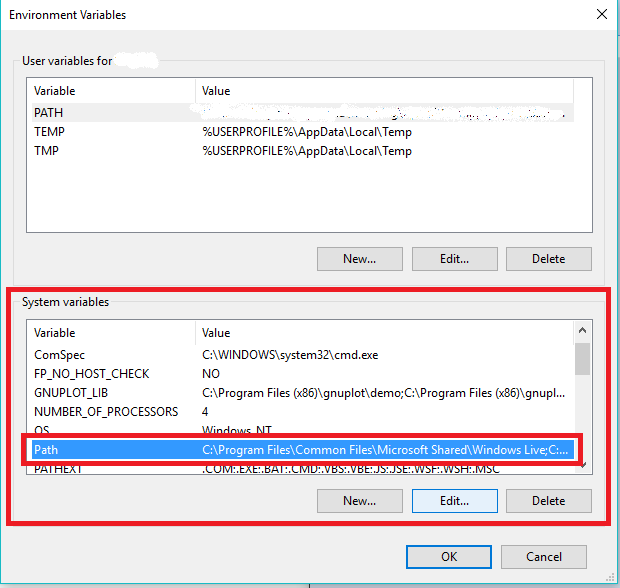
\includegraphics[height=8cm]{004.png}\\
		\linebreak
		Select Path, click Edit
		\pagebreak
		\item Step:5	\linebreak
		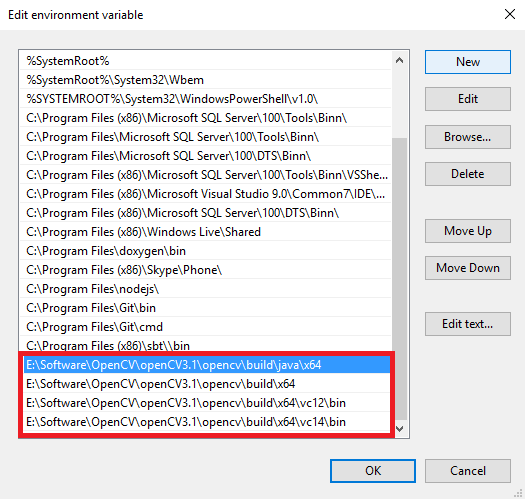
\includegraphics[height=8cm]{005.png}\\
		\linebreak
		Select New, enter the paths to the above folders which may be located in the given
		OpenCV files, restart computer to take effect.
	\end{itemize}
	
	\section{Using The System}
	\subsection{OpenCV}
	\subsubsection{What is it?}
	OpenCV is the open source software which was selected and provides the framework
	utilized by the Smart Image Identifier software.
	\subsubsection{Why was it used?}
	Just one of the things many things OpenCV is capable of is that it provides libraries and
	functionality to assist in the detection of humans within images.

	\subsection{Classes}
	\subsubsection{PeopleDetect}
	This is the class which Smart Image Identifier was implemented.
	Full Doxygen commenting is provided in this class, describing functions, their parameters
	and a brief description on its purpose.
	\subsubsection{Writer}
This class provides us with video writing capabilities, it was used to create a copy of the
video in question.
\subsubsection{FourCC}
This class provides us with a “four character code” (4CC) which is used by AVI files.
It wraps a 32-bit value to be used as a 4CC inside an AVI file, so that it is guaranteed to be
valid, and it incurs no overhead if used repeatedly.

\subsubsection{Database}
This class is responsible for all database related processing: retrieving an image, decoding an image as well as any other required data handling regarding the database.

\subsection{Functions}
\subsubsection{greyscale(BufferedImage image, Mat mat)}
This method receives two parameters, image and mat. The image variable is used to
create a temporary mat object with the same dimensions whereas the mat object is used
to transfer the data within the image after which is grey-scaled and returned.
Grey-scaling assists in image processing by removing all the colour the image holds less
data therefor becomes easier to process.
\subsubsection{equalization(BufferedImage image, Mat mat)}
This method receives two parameters: image and mat. The image variable is used to
create a temporary mat object with the same dimensions whereas the mat object is used
to transfer the data within the image which is required to be grey-scaled.
This increased the contrast within the image helping objects to appear more defined in
the image.
\subsubsection{enlargeImage(BufferedImage image, Mat mat)}
This method receives two parameters: image and mat. The image variable is used to
create a temporary mat object with the same dimensions whereas the mat object is used
to transfer the data within the image.
This method enlarges an image, it helps with identification of objects as the windows of
pixels processed making it easier to detect.
\subsubsection{generateMat(BufferedImage image)}
This method receives one parameter: image. The image variable is used to create a mat
object with the same dimensions which is returned to the system and stored for
processing.
\subsubsection{generateImage(BufferedImage image, Mat mat, byte[] data)}
This method receives three parameters: image, mat and byte. The image variable is used
for identifying sizes, the Mat object holds the data which is to be saved into an image and
data which holds additional data containing the location of the boxes which are drawn
onto the image after a human is detected.
This method outputs the results of the Smart Image Identifier and saves it as a JPG file
which is stored in the output folder within the project.
\subsubsection{processImage(String url)}
This method receives one parameter: url. The url is the location of an image which is
required to be processed.
This method is the heart of Smart Image Identifier, all the processing required for human
detection is done here.
\subsubsection{runTests(String url)}
This method receives one parameter: url. The url is the location of an image which is required to be processed.
This method runs the image through various tests.

\subsubsection{readDatabase()}
This method connects to the Willburg database, retrieving images for processing
\subsubsection{getImage(byte[] base64String)}
This method connects receives one parameter: base64String. This string contains base64 encryption used to store the image in the database which is then used to create an image which in turn is pushed forward for processing.
\pagebreak
\section{Troubleshooting}
The system has no human interaction, it is simply a stable communication line between two systems which is required to be maintained.

\end{document}
